\documentclass[11pt,a4paper,oneside]{article}
\usepackage[a4paper,top=2cm,bottom=2.5cm,left=1.8cm,right=1.8cm]{geometry}
\usepackage[T1]{fontenc}
\usepackage[utf8]{inputenc}
\usepackage[italian]{babel}
\usepackage{frontespizio}
\usepackage{graphicx}
\usepackage{subfig}
\usepackage[italian]{varioref}
\usepackage{url}

\begin{document}
\baselineskip 22pt

%Indice%
\tableofcontents\thispagestyle{empty}\clearpage

\section{Introduzione}
\pagenumbering{arabic}
\baselineskip 12pt
Negli ultimi anni c'è stato un discreto aumento dell'occupazione femminile in Italia che, da poco più del 33\% nell'anno '77, è arrivata nel 2019 a superare il 50\%. Per quanto il miglioramento sia da apprezzare, la metà della popolazione femminile è ancora da considerarsi disoccupata, e anche se la maggior parte in questa percentuale è probabile che siano le donne più giovani, ancora dietro agli studi, è necessario che il tasso continui ad aumentare. A livello europeo, infatti, il nostro paese si trova tra gli ultimi posti per quanto riguarda il tasso di occupazione femminile, mantenendo un forte divario tra uomini e donne, e di conseguenza privandosi di un'importante componente lavorativa.

In questo studio, cerchiamo di analizzare l'andamento del tasso preso in considerazione, per arrivare a una previsione di come muterà nel futuro prossimo.

\section{Tabella dei dati}
La tabella è stata recuperata dal sito \url{http://dati.istat.it/Index.aspx?DataSetCode=DCCV_TAXOCCU1}, selezionando i dati disponibili relativi al sesso femminile, alla fascia di età 15-64 anni, per ogni trimestre da gennaio del 1977 a settembre del 2019. Il dataset è stato esportato in formato csv, e sono stati prese in considerazione soltanto le colonne indicanti il trimestre e il tasso occupazionale relativo. Sono presenti in tutto 171 osservazioni.\\
Dopo aver importato sul software il file csv, effettuiamo la conversione dei dati in serie storica:
\begin{verbatim}
> to.data = read.csv("tabella.csv",row.names=1)
> head(to.data)
> to = ts(to.data,frequency=4,start=c(1977))
\end{verbatim}
Siamo adesso pronti per il nostro studio.
\section{Analisi dei dati}
Iniziamo con la visualizzazione della nostra serie storica nella figura~\ref{fig:tsplot}: possiamo subito notare la presenza di un forte trend ascendente, mentre non è molto evidente una stagionalità.  Di fatto, se osserviamo attentamente, possiamo vedere che le fluttuazioni della serie nel grafico, identificate dai lievi picchi, sono tutte in corrispondenza di un anno solare. Soprattutto nei primi anni disponibili, fino almeno al 2000, i picchi sembrano molto simili tra loro, indicando quindi che una stagionalità, seppur probabilmente di ordine di grandezza piccolo, deve essere presente.
\begin{figure}[h]
\centering
\subfloat[][\emph{Visualizzazione dell'andamento dei dati}\label{fig:tsplot}]
{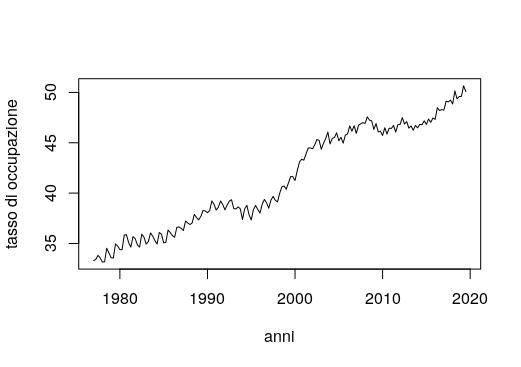
\includegraphics[width=0.5\textwidth]{images/tsplot}}
\subfloat[][\emph{Funzione di autocorrelazione}\label{fig:acf}]
{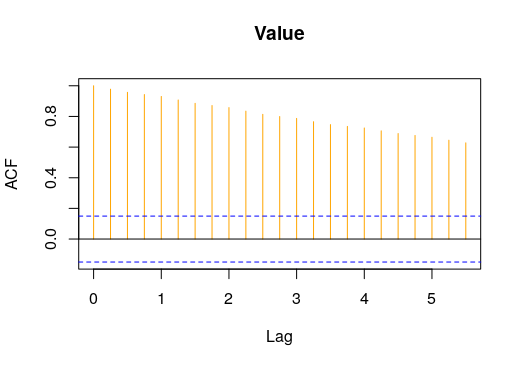
\includegraphics[width=0.5\textwidth]{images/acf}} \\
\caption{}
\label{fig:grafici}
\end{figure}

Andiamo, quindi, ad analizzare la funzione di autocorrelazione e anche da essa vediamo che la componente di periodicità sembra non esserci (fig.~\ref{fig:tsplotDiff}). Sappiamo, però, che questa funzione è di dubbia interpretazione se in presenza di un forte trend, e proviamo quindi a visualizzare la serie al netto del trend: 
\begin{verbatim}
> plot(diff(to))
> acf(diff(to),col="orange")
\end{verbatim}
Si nota già meglio che ogni anno è visualizzato da un picco, sottolineando quindi la presenza di stagionalità. Come già detto, questi picchi sono ben distinti per i primi anni, almeno fino al 2003, per poi cambiare andamento e suddividersi in picchi più confusi tra i vari trimestri. Dalla funzione di autocorrelazione, poi, sembra che così una componente stagionale possa essere effettivamente presente: in corrispondenza dell'inizio di ogni periodo, vediamo che il valore di \textit{acf} si staglia al di sopra degli altri valori, evento che era stato mascherato nei grafici precedenti dalla presenza del trend accentuato.
\begin{figure}[h]
\centering
\subfloat[][\emph{Visualizzazione dei dati al netto del trend}\label{fig:tsplotDiff}]
{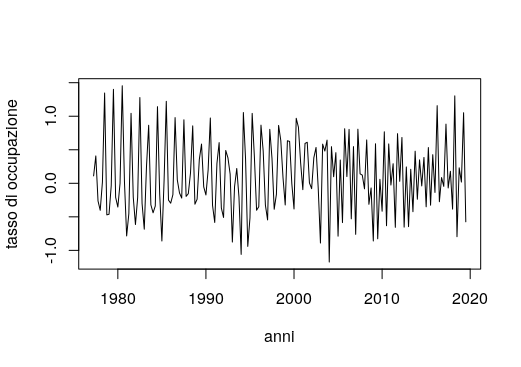
\includegraphics[width=0.5\textwidth]{images/tsplotDiff}}
\subfloat[][\emph{Funzione di autocorrelazione al netto del trend}\label{fig:acfDiff}]
{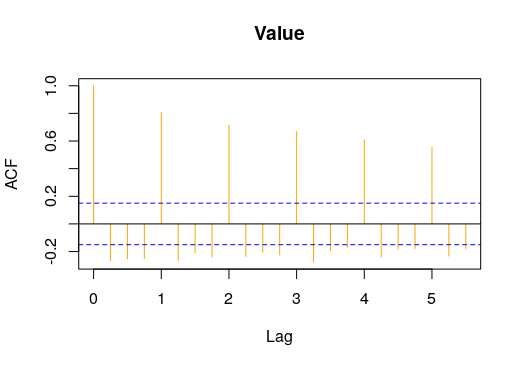
\includegraphics[width=0.5\textwidth]{images/acfDiff}} \\
\caption{}
\label{fig:graficiDiff}
\end{figure}

Proviamo, ora, a visualizzare l'andamento annuale della serie, sovrapponendo i valori a disposizione di ogni anno (fig.~\ref{fig:plotPeriodi}). Sembra ancora che ci sia una lieve periodicità, per cui verso la metà di ogni anno il tasso sembra crescere per poi riabbassarsi leggermente: questo fenomeno, dovuto probabilmente alla richiesta maggiore di lavoro durante la stagione estiva, così come alla fine dell'anno per le feste natalizie, si registra con fluttuazioni a livelli di cifre decimali nel tasso registrato ogni trimestre, e per questo motivo non viene facilmente distinto.
\begin{figure}[h]
\centering
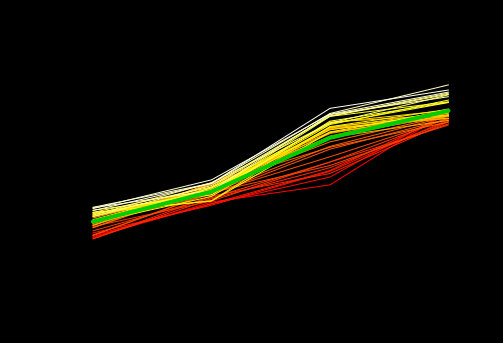
\includegraphics[width=0.4\textwidth]{images/plotPeriodi}
\caption{Andamento annuale della serie}
\label{fig:plotPeriodi}
\end{figure}

\subsection{Decomposizione della serie}
Andando avanti con la nostra analisi, effettuiamo la decomposizione della serie nelle componenti di trend, stagionalità e rumore (fig.~\ref{fig:decompose}). Si vede, ancora, che il fenomeno principale della serie è il trend, che ha un andamento crescente, mentre la componente di stagionalità ha ampiezza minore del rumore (fig.~\ref{fig:seasNoise}).
Sembra, quindi, che la periodicità dei valori della serie, dovuta ai cambi di stagione, sia da trascurare in confronto all'aumento del tasso di occupazione che è stato registrato di anno in anno. 
\begin{figure}[h]
\centering
\subfloat[][\emph{Decomposizione della serie}\label{fig:decompose}]
{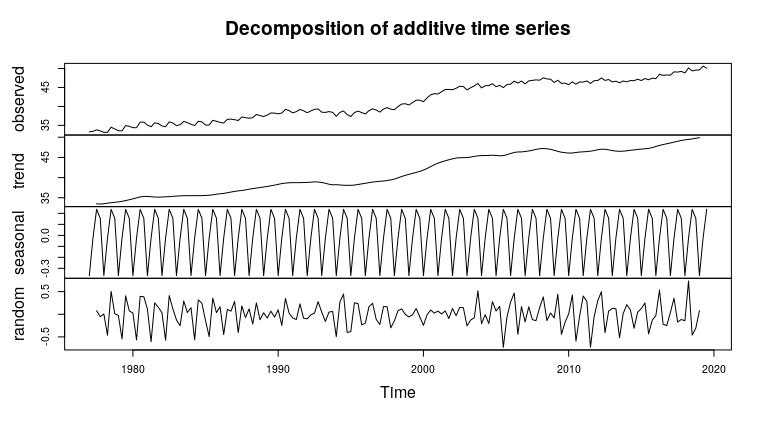
\includegraphics[width=0.5\textwidth]{images/decompose}}
\subfloat[][\emph{Confronto tra componente di stagionalità e di rumore}\label{fig:seasNoise}]
{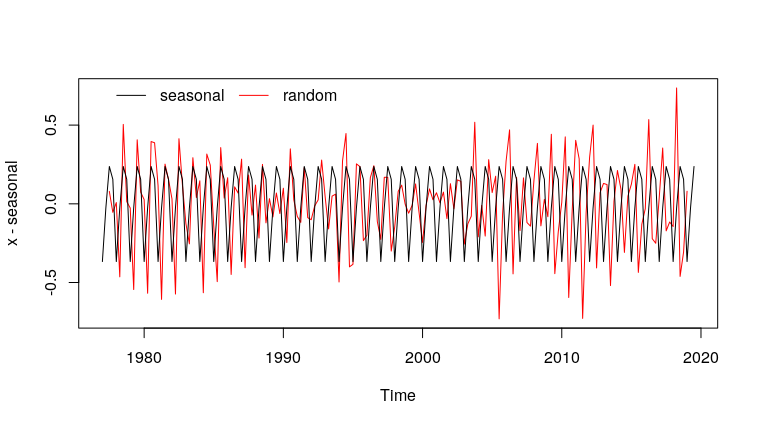
\includegraphics[width=0.5\textwidth]{images/seasNoise}} \\
\caption{}
\label{fig:graficiDiff}
\end{figure}

\subsection{Smorzamento esponenziale}
Applichiamo il metodo dello smorzamento esponenziale (SE) sulla serie, seguito dallo smorzamento esponenziale con trend (SET), per procedere con l'analisi.
Sembra che entrambi i metodi, riescano a catturare abbastanza bene l'andamento della serie.
Cerchiamo di catturare solo la componente di trend della serie storica, andando a modificare i parametri del metodo:
\begin{verbatim}
> plot(to.set)
> points(HoltWinters(to,alpha=0.1,beta=0.01,gamma=F)$fitted,col="blue",type="l")
\end{verbatim}
\begin{figure}[h]
\centering
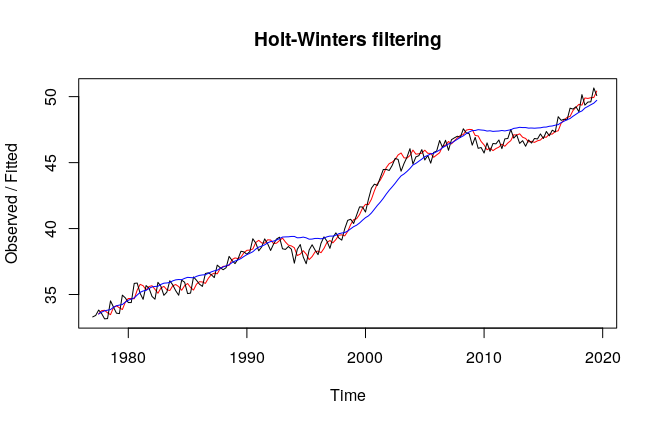
\includegraphics[width=0.5\textwidth]{images/trend}
\caption{SET con parametri settati a mano per catturare il trend}
\label{fig:trend}
\end{figure}

Andando ad analizzare, invece, la capacità predittiva dei due modelli, vediamo che manca la componente di stagionalità che, seppur minima, è decisiva per distinguere i vari trimestri, soprattutto a livello di predizione del prossimo futuro.

Ci concentriamo, così, sul metodo dello smorzamento esponenziale che considera sia trend che stagionalità, detto anche metodo di Holt-Winters:
\begin{verbatim}
> to.hw=HoltWinters(to)
> plot(to.hw,lwd=2)
\end{verbatim}
Il grafico risultante, che si trova in figura~\ref{fig:hw}, fa notare che l'andamento della serie è molto ben catturato da questo modello. 
\begin{figure}[h]
\centering
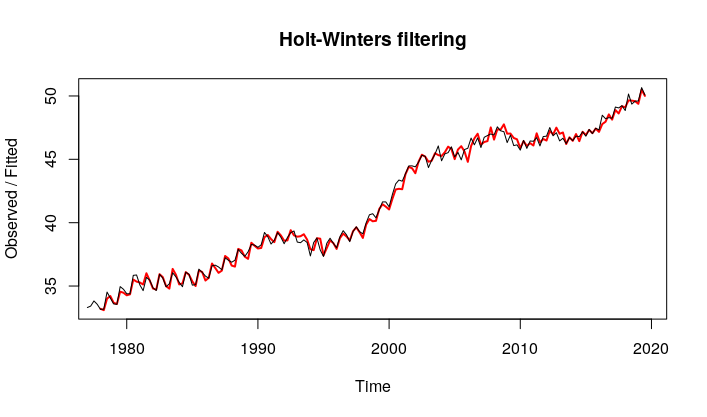
\includegraphics[width=0.6\textwidth]{images/hw}
\caption{Smorzamento esponenziale con trend e con stagionalità}
\label{fig:hw}
\end{figure}

Proviamo, inoltre, a effettuare una previsione dei valori del prossimo anno, ottenendo risultati decisamente attendibili (fig.~\ref{fig:hwPrevisioni}), mentre provando a prevedere l'andamento del tasso di occupazione per più anni il risultato non è esaltante, visto che la previsione del primo anno viene ripetuta altre due volte, un po’ traslata verso l'alto, seguendo un trend del tutto lineare. 
\begin{figure}[h]
\centering
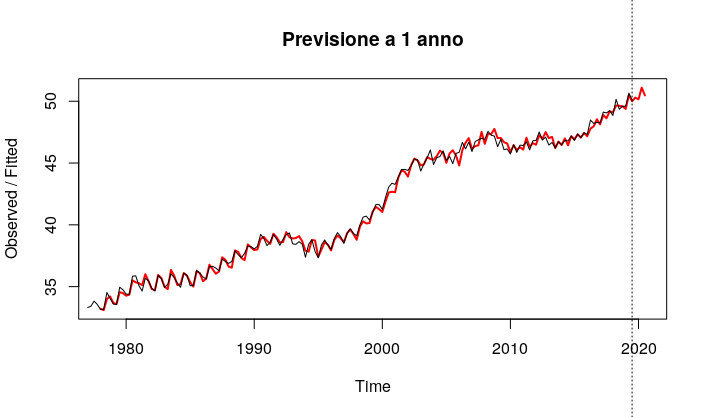
\includegraphics[width=0.6\textwidth]{images/hwPrevisioni}
\caption{Smorzamento esponenziale con previsione}
\label{fig:hwPrevisioni}
\end{figure}

\subsection{Estrazione dei residui}
Procediamo ad analizzare i residui del modello costruito con il metodo di Holt-Winters, per vedere se in essi è rimasta una struttura o se possano essere considerati con buona approssimazione gaussiani.
\begin{verbatim}
> to.hw.r=as.vector(residuals(to.hw))
> plot(to.hw.r,pch=20)
> 1 - var(to.hw.r)/var(to)
          Value
Value 0.9959087
\end{verbatim}

La varianza spiegata ottenuta, uguale al 99\% è molto soddisfacente. Guardando la funzione di autocorrelazione si nota una periodicità, segno che i residui mantengono parte della componente stagionale della serie.
Comunque, dal grafico dei residui in figura~\ref{fig:hwResid}, si nota che essi sono abbastanza sparsi. 
Portando avanti la loro analisi, vediamo che l'istogramma è molto simile a quello di una distribuzione gaussiana con stessa media e deviazione standard. Anche il grafico quantile-quantile è abbastanza buono, con la maggior parte dei punti aderenti alla retta ottimale, soprattutto al centro, mentre le code si discostano di poco (fig.~\ref{fig:residAnalysis}). Effettuando, infine, il test di Shapiro-Wilk si ottiene un valore praticamente uguale a quello di una distribuzione gaussiana della stessa dimensione:
\begin{verbatim}
> shapiro.test(to.hw.r)
	Shapiro-Wilk normality test
data:  to.hw.r
W = 0.99263, p-value = 0.5561
> shapiro.test(rnorm(167))
	Shapiro-Wilk normality test
data:  rnorm(167)
W = 0.99369, p-value = 0.6896
\end{verbatim}
Tutti questi fattori indicano che i residui del modello costruito sono vicini a essere casuali, ma mantengono una parte strutturale dei dati: il modello è da considerare abbastanza soddisfacente.
\begin{figure}[h]
\centering
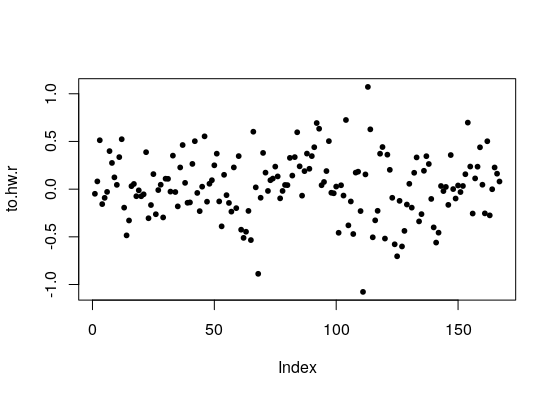
\includegraphics[width=0.5\textwidth]{images/hwResid}
\caption{Residui del modello costruito con il metodo di Holt-Winters}
\label{fig:hwResid}
\end{figure}
\begin{figure}[h]
\centering
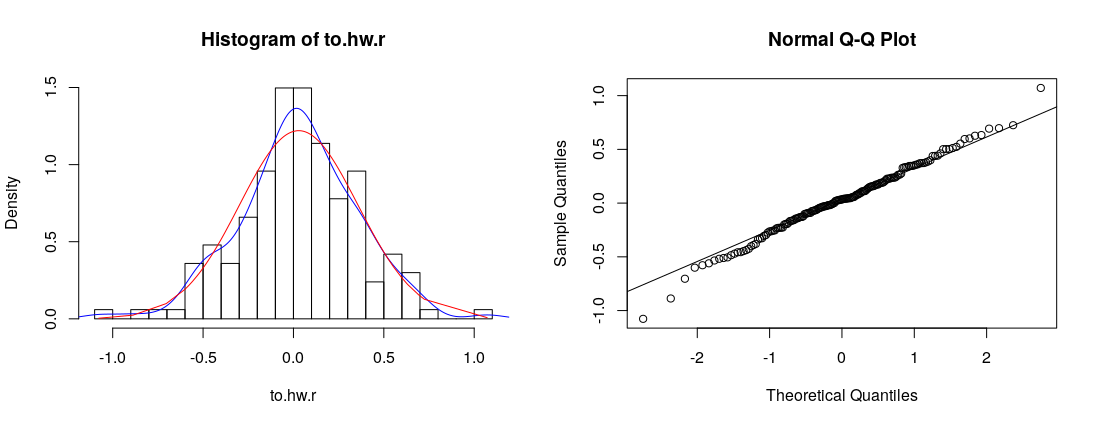
\includegraphics[width=1\textwidth]{images/residAnalysis}
\caption{Analisi dei residui}
\label{fig:residAnalysis}
\end{figure}

\subsection{Incertezza delle previsioni}
Vediamo come utilizzare i residui per valutare l'incertezza di eventuali previsioni future. Calcoliamo un intervallo di confidenza al 90\% sulle previsioni future:
\begin{verbatim}
> quantile(to.hw.r,0.05)
        5% 
-0.5091299 
> quantile(to.hw.r,0.95)
      95% 
0.5444803
> predict(to.hw,1) + quantile(to.hw.r,0.05)
         Qtr4
2019 49.78653
> predict(to.hw,1) + quantile(to.hw.r,0.95)
         Qtr4
2019 50.84014
\end{verbatim}
ottenendo un intervallo più o meno incentrato in zero. Per la visualizzazione grafica dell'intervallo di confidenza delle previsioni, si può osservare la figura~\ref{fig:confidenza}.
\begin{figure}[h]
\centering
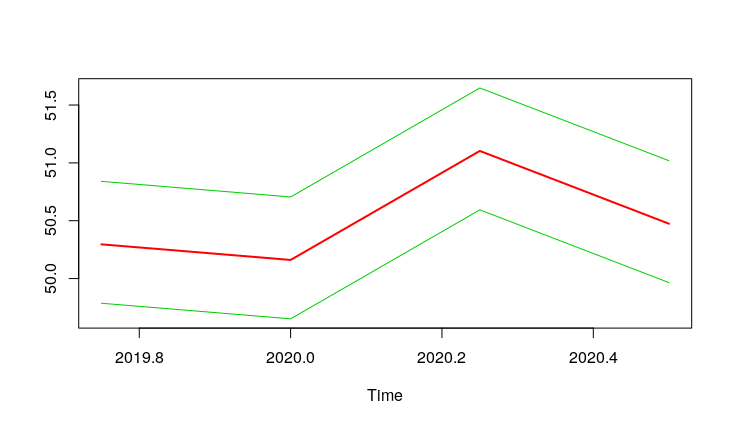
\includegraphics[width=0.6\textwidth]{images/confidenza}
\caption{Intervallo di confidenza delle previsioni future}
\label{fig:confidenza}
\end{figure}

\subsection{Autovalidazione}
Valutiamo, infine, la bontà del modello di smorzamento esponenziale con trend e stagionalità, andando a testarne la capacità di predizione tramite una procedura di autovalidazione. Cerchiamo, quindi, di predire gli ultimi quattro valori della nostra serie, per poi andare a confrontarli con i valori reali: otteniamo dei risultati con un errore di predizione pari al 20\%, non molto soddisfacente (fig.~\ref{fig:prediction}). 
\begin{verbatim}
> sqrt(var(pred-real)/var(real))
[1] 0.1967183
\end{verbatim}
\begin{figure}[h]
\centering
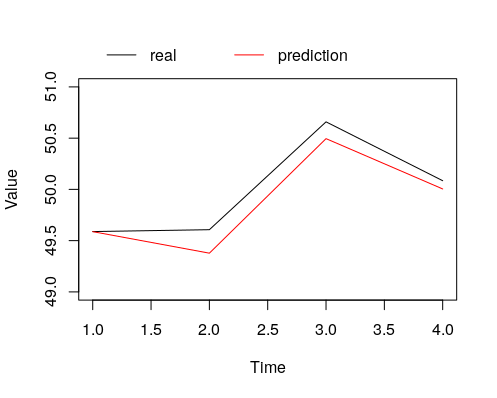
\includegraphics[width=0.5\textwidth]{images/prediction}
\caption{Predizioni effettuate dal modello, a confronto con i dati reali}
\label{fig:prediction}
\end{figure}

\section{Conclusioni}

\end{document}